\documentclass[acmsmall,review,anonymous]{acmart}

% Package imports
\usepackage{booktabs}
\usepackage{multirow}
\usepackage{graphicx}
\usepackage{amsmath}
\usepackage{algorithm}
\usepackage{algorithmic}
\usepackage{url}
\usepackage{hyperref}
\usepackage{tikz}
\usepackage{pgfplots}
\usepackage{balance}

% ACM-specific formatting
\acmVolume{1}
\acmNumber{1}
\acmArticle{1}
\acmYear{2025}
\acmMonth{10}
\acmDOI{10.1145/XXXXXXX}

% Copyright
\acmYear{2025}
\acmDOI{10.1145/XXXXXXX}

% Authors
\acmBooktitle{ACM Transactions on Recommender Systems}
\acmPrice{15.00}
\acmISBN{978-1-4503-XXXX-X/25/10}

\title{Implicit vs. Explicit Feedback in Recommender Systems: A Comprehensive Survey}
\author{Your Name}
\affiliation{%
  \institution{Affiliation}
  \streetaddress{Street Address}
  \city{City}
  \state{State}
  \postcode{Postcode}
  \country{Country}}
\email{email@domain.com}

% CCS Concepts
\ccsdesc[500]{Information systems~Recommender systems}
\ccsdesc[500]{Information systems~Personalization}
\ccsdesc[300]{Computing methodologies~Neural networks}
\ccsdesc[300]{Information systems~Information retrieval}

\keywords{Recommender Systems, Implicit Feedback, Explicit Feedback, Machine Learning, Evaluation Metrics}

\begin{document}

\begin{abstract}
Recommender systems have become integral to modern digital platforms, leveraging user feedback to personalize content and enhance user experience. This comprehensive survey provides an in-depth analysis of implicit and explicit feedback mechanisms in RS, highlighting their differences, modeling approaches, evaluation methodologies, and practical implications across diverse domains. Implicit feedback, derived from user behaviors such as clicks, views, and purchases, offers abundant data but introduces challenges like noise and sparsity. Explicit feedback, including ratings and reviews, provides clearer user preferences but suffers from low response rates and potential biases.

We present a detailed taxonomy of feedback types, encompassing sources, properties, and collection mechanisms, along with privacy considerations. The survey reviews learning paradigms from classical matrix factorization and collaborative filtering to advanced deep learning, reinforcement learning, and contrastive learning approaches. Hybrid models that integrate both feedback types are thoroughly examined. Evaluation methodologies are discussed, including standard metrics, biases in datasets, and user behavior interpretations. Applications across e-commerce, news, music, video streaming, and social media are explored, emphasizing how feedback types influence personalization and explainability.

Key challenges such as feedback sparsity, noise handling, user intent disambiguation, cold-start problems, and cross-domain learning are identified. Emerging directions, including feedback-aware fairness, contextual modeling, privacy-preserving techniques, and large language model-based feedback interpretation, are highlighted. A comparative analysis with detailed tables summarizes methods, datasets, metrics, and feedback types. The survey concludes with a visionary outlook on future RS that balance implicit and explicit feedback using self-supervised and multimodal approaches.

By synthesizing over a decade of research (2010--2025), this work aims to guide researchers and practitioners in developing more robust, fair, and interpretable recommender systems. The survey includes over 50 citations to seminal and recent works, providing a foundational reference for the field.
\end{abstract}

\maketitle

\section{Introduction}
\label{sec:intro}

Recommender systems (RS) have evolved from simple collaborative filtering algorithms to sophisticated machine learning pipelines that power personalized experiences across digital platforms. These systems analyze user preferences to suggest relevant items, playing a pivotal role in e-commerce, entertainment, social media, and content platforms. The effectiveness of recommender systems fundamentally depends on the quality, quantity, and type of user feedback utilized for learning user preferences and item characteristics.

The landscape of user feedback in recommender systems is traditionally bifurcated into two primary categories: \textit{implicit feedback} and \textit{explicit feedback}. This dichotomy represents not just different data collection mechanisms, but fundamentally different approaches to understanding user preferences, each with distinct advantages, limitations, and modeling requirements.

\textbf{Implicit feedback} encompasses user behaviors that indirectly reveal preferences without requiring conscious effort from users. These signals include clicks, views, dwell times, purchases, shares, and other interaction patterns automatically captured by digital systems. The abundance of implicit feedback makes it particularly attractive for large-scale applications, but its inherent ambiguity and noise present significant modeling challenges.

\textbf{Explicit feedback}, in contrast, involves direct, intentional expressions of user preferences through ratings, reviews, likes, dislikes, and other deliberate inputs. While explicit feedback provides clearer, more interpretable signals about user tastes, it suffers from low participation rates and potential biases due to the effort required from users.

\subsection{Historical Evolution of Feedback in Recommender Systems}

The evolution of feedback utilization in recommender systems reflects broader trends in machine learning and user interface design:

\subsubsection{Early Era (1990s--2000s): Explicit Feedback Dominance}
Early recommender systems, such as GroupLens and the original Netflix Prize, relied heavily on explicit ratings. The collaborative filtering paradigm, pioneered by the GroupLens project at the University of Minnesota, established explicit ratings as the gold standard for preference learning. During this period, research focused on matrix factorization techniques that could handle sparse rating matrices, with methods like Singular Value Decomposition (SVD) and neighborhood-based approaches dominating the field.

\subsubsection{Mid Era (2010s): Implicit Feedback Revolution}
The rise of web-scale applications brought implicit feedback to the forefront. Companies like Amazon and Netflix began leveraging clickstream data, purchase histories, and viewing behaviors. This shift was driven by data abundance rather than data quality, leading to the development of implicit feedback-specific algorithms like Weighted Matrix Factorization and Bayesian Personalized Ranking (BPR).

\subsubsection{Current Era (2020s): Hybrid and Multimodal Approaches}
Modern recommender systems increasingly integrate multiple feedback types, incorporating contextual information, multimodal signals, and advanced machine learning techniques. The emergence of deep learning, reinforcement learning, and large language models has enabled more sophisticated feedback processing, while privacy concerns have driven the development of federated and differential privacy approaches.

\subsection{The Feedback Spectrum: Beyond Binary Classification}

While the implicit-explicit dichotomy provides a useful framework, real-world feedback exists on a spectrum with varying degrees of explicitness and implicitness:

\subsubsection{Quasi-Explicit Feedback}
Some feedback mechanisms blur the boundary between implicit and explicit. For example:
\begin{itemize}
    \item \textbf{Thumbs up/down}: Simple binary choices that are more explicit than clicks but less effortful than detailed ratings
    \item \textbf{Star ratings with half-stars}: Provide more granularity than binary feedback but less cognitive load than written reviews
    \item \textbf{Preference rankings}: Users rank items relative to each other, providing comparative feedback
\end{itemize}

\subsubsection{Behavioral Implicit Feedback}
Implicit feedback itself encompasses various behavioral signals:
\begin{itemize}
    \item \textbf{Navigation patterns}: Mouse movements, scroll depth, and time spent on pages
    \item \textbf{Physiological signals}: Heart rate, eye tracking, and facial expressions (emerging with wearable devices)
    \item \textbf{Social behaviors}: Following, unfollowing, and network interactions
\end{itemize}

\subsubsection{Multimodal Feedback Integration}
Modern systems combine multiple feedback modalities:
\begin{itemize}
    \item \textbf{Textual feedback}: Reviews, comments, and search queries
    \item \textbf{Visual feedback}: Image uploads, video reactions, and visual preferences
    \item \textbf{Audio feedback}: Voice commands, music preferences, and audio reactions
\end{itemize}

\subsection{Why Feedback Types Matter: Theoretical Foundations}

The choice of feedback type has profound implications for system design, user experience, and algorithmic performance:

\subsubsection{Information Theory Perspective}
From an information theory standpoint, implicit feedback provides high-volume, low-fidelity signals, while explicit feedback offers low-volume, high-fidelity information. The optimal feedback strategy involves maximizing information gain per user interaction.

\subsubsection{Cognitive Psychology Perspective}
Explicit feedback requires conscious reflection and effort, engaging System 2 thinking in Daniel Kahneman's framework. Implicit feedback captures System 1 automatic responses, providing insights into instinctive preferences but requiring careful interpretation.

\subsubsection{Economic Perspective}
Implicit feedback has near-zero marginal cost for collection but high processing costs. Explicit feedback incurs user effort costs but lower computational costs for interpretation.

\subsection{Current Research Landscape and Gaps}

Despite extensive research, several critical gaps persist:

\subsubsection{Unified Theoretical Framework}
There is no comprehensive theoretical framework that explains when and why different feedback types should be used, or how they interact in hybrid systems.

\subsubsection{Cross-Domain Feedback Transfer}
Understanding how feedback learned in one domain (e.g., movies) can transfer to another (e.g., books) remains underexplored.

\subsubsection{Longitudinal Feedback Dynamics}
How user feedback patterns evolve over time, and how systems should adapt to changing preference landscapes, is not well understood.

\subsubsection{Fairness and Bias in Feedback Collection}
The differential availability and quality of feedback across demographic groups creates fairness challenges that are only beginning to be addressed.

\subsubsection{Privacy-Efficiency Trade-offs}
Balancing the benefits of rich feedback collection with privacy preservation requirements remains a key challenge.

\subsection{Key Research Questions}
\label{subsec:research_questions}

To address these gaps, we pose the following comprehensive research questions:

\begin{enumerate}
    \item \textbf{Fundamental Characteristics}: How do implicit and explicit feedback differ in terms of data characteristics, collection mechanisms, and inherent biases? What are the theoretical bounds on performance for each feedback type?

    \item \textbf{Modeling Paradigms}: What are the most effective algorithms for modeling each feedback type? How can we develop unified frameworks that handle both types seamlessly?

    \item \textbf{Hybrid Integration}: What are the optimal strategies for combining implicit and explicit feedback? How can we resolve conflicts between different feedback signals?

    \item \textbf{Evaluation Frameworks}: How should we evaluate systems that use different feedback types? What metrics account for the unique characteristics of each feedback modality?

    \item \textbf{Domain Adaptation}: How do feedback characteristics and optimal modeling approaches vary across different application domains?

    \item \textbf{Bias and Fairness}: How can we mitigate biases inherent in different feedback collection mechanisms? What fairness guarantees can we provide?

    \item \textbf{Privacy Preservation}: How can we collect and utilize feedback while preserving user privacy? What are the trade-offs between utility and privacy?

    \item \textbf{Temporal Dynamics}: How do feedback patterns evolve over time? How should systems should adapt to changing user preferences and feedback landscapes?

    \item \textbf{Emerging Technologies}: What role will large language models, multimodal learning, and brain-computer interfaces play in future feedback systems?

    \item \textbf{Human-AI Interaction}: How can recommender systems elicit better feedback from users? What interfaces and interaction designs optimize feedback quality and quantity?
\end{enumerate}

\subsection{Scope and Contributions}

This survey provides a comprehensive examination of implicit and explicit feedback in recommender systems, covering:

\begin{itemize}
    \item \textbf{Comprehensive Taxonomy}: A detailed classification of feedback types, sources, and properties with visual representations and examples.

    \item \textbf{Modeling Landscape}: An extensive review of algorithms from classical matrix factorization to cutting-edge deep learning and reinforcement learning approaches.

    \item \textbf{Evaluation Frameworks}: Detailed evaluation methodologies, metrics, and bias analyses specific to different feedback types.

    \item \textbf{Domain Applications}: In-depth case studies across e-commerce, entertainment, social media, and emerging domains.

    \item \textbf{Technical Challenges}: Identification and analysis of core challenges including sparsity, noise, bias, and privacy.

    \item \textbf{Future Directions}: Visionary outlook on emerging technologies and research directions for the next decade.

    \item \textbf{Practical Guidance}: Comparative analyses, best practices, and implementation considerations for practitioners.
\end{itemize}

\subsection{Paper Organization}

The remainder of this paper is structured as follows: Section~\ref{sec:taxonomy} presents a comprehensive taxonomy of feedback types with detailed classifications and properties. Section~\ref{sec:learning} reviews learning paradigms and modeling approaches, from classical to modern techniques. Section~\ref{sec:evaluation} discusses evaluation methodologies and metrics. Section~\ref{sec:applications} explores applications across diverse domains with case studies. Section~\ref{sec:challenges} identifies challenges and open research directions. Finally, Section~\ref{sec:summary} provides comparative analyses and future outlook.

\subsection{Methodology and Literature Review Approach}

This survey synthesizes research from over 15 years (2008--2024), drawing from major conferences (RecSys, SIGIR, KDD, WWW) and journals (ACM TORS, IEEE TKDE, JMLR). We prioritize recent work (2020+) while providing historical context. Our analysis combines theoretical insights with empirical evidence, emphasizing practical implications for system design and deployment.

\section{Taxonomy of Feedback Types}
\label{sec:taxonomy}

Feedback in recommender systems can be categorized based on its source, properties, and collection mechanisms. We develop a comprehensive taxonomy that encompasses both implicit and explicit feedback, considering behavioral signals, data characteristics, and privacy implications. This taxonomy goes beyond simple binary classification to capture the nuanced spectrum of feedback modalities available in modern recommender systems.

\subsection{Feedback Sources and Granularity Levels}

\subsubsection{Implicit Feedback Sources}
Implicit feedback originates from user actions that indirectly reveal preferences without requiring conscious user effort. These signals are automatically captured through digital interactions and provide rich behavioral data.

\paragraph{Micro-level Implicit Signals}
\begin{itemize}
    \item \textbf{Clickstream data}: Individual clicks on items, links, or recommendations. Includes metadata like click position, time of day, and device type.
    \item \textbf{Dwell time}: Duration spent viewing an item page or content. Thresholds (e.g., 30\% of video watched) indicate engagement levels.
    \item \textbf{Scroll depth}: How far users scroll through content, revealing interest intensity.
    \item \textbf{Mouse movements}: Cursor trajectories and hover behaviors that indicate attention patterns.
    \item \textbf{Keyboard interactions}: Search queries, typing patterns, and navigation shortcuts.
\end{itemize}

\paragraph{Meso-level Implicit Signals}
\begin{itemize}
    \item \textbf{Session-level behaviors}: Sequences of page views, item comparisons, and navigation paths within a single session.
    \item \textbf{Purchase funnels}: Cart additions, wishlists, and abandoned checkout behaviors.
    \item \textbf{Social engagement}: Shares, bookmarks, saves, and forwarding actions.
    \item \textbf{Consumption patterns}: Reading completion rates, playback speeds, and repeat consumption.
\end{itemize}

\paragraph{Macro-level Implicit Signals}
\begin{itemize}
    \item \textbf{Longitudinal patterns}: Repeated purchases, seasonal preferences, and evolving taste profiles.
    \item \textbf{Cross-platform behaviors}: Consistent preferences across different devices and platforms.
    \item \textbf{Network effects}: Influence from social connections and community behaviors.
\end{itemize}

\subsubsection{Explicit Feedback Sources}
Explicit feedback involves deliberate user actions to express preferences, requiring conscious effort but providing clearer semantic meaning.

\paragraph{Quantitative Explicit Feedback}
\begin{itemize}
    \item \textbf{Numerical ratings}: Star ratings (1-5 scale), percentage scores, or continuous scales.
    \item \textbf{Like/dislike binaries}: Simple positive/negative indicators with minimal cognitive load.
    \item \textbf{Preference rankings}: Ordinal rankings of items relative to each other.
    \item \textbf{Confidence scores}: Self-assessed confidence in one's own ratings.
\end{itemize}

\paragraph{Qualitative Explicit Feedback}
\begin{itemize}
    \item \textbf{Textual reviews}: Written opinions, critiques, and detailed feedback.
    \item \textbf{Tags and categories}: User-assigned labels and classifications.
    \item \textbf{Feature ratings}: Specific aspect ratings (e.g., "sound quality: 4/5, plot: 3/5").
    \item \textbf{Comparative feedback}: Direct comparisons between items or against expectations.
\end{itemize}

\paragraph{Interactive Explicit Feedback}
\begin{itemize}
    \item \textbf{Conversational feedback}: Dialogue-based preference elicitation through chat interfaces.
    \item \textbf{Preference surveys}: Structured questionnaires and preference profiling.
    \item \textbf{Active learning queries}: System-initiated questions to clarify user preferences.
\end{itemize}

\subsection{Feedback Properties and Characteristics}

Feedback types exhibit distinct properties that influence their utility, reliability, and modeling requirements. Understanding these properties is crucial for designing appropriate algorithms and evaluation metrics.

\subsubsection{Data Abundance and Collection Dynamics}

\begin{table}[h]
\centering
\caption{Comparative Analysis of Feedback Properties}
\label{tab:feedback_properties_detailed}
\begin{tabular}{@{}lcccc@{}}
\toprule
Property & Implicit Feedback & Explicit Feedback & Hybrid Approaches & Key Implications \\
\midrule
Data Volume & Very High & Low-Moderate & High & Scalability trade-offs \\
Collection Cost & Near Zero & High (User Effort) & Variable & Economic considerations \\
Temporal Resolution & Real-time & Delayed & Mixed & Adaptation speed \\
Semantic Clarity & Low & High & Moderate & Interpretation complexity \\
Noise Level & High & Low-Moderate & Moderate & Signal processing needs \\
Sparsity Pattern & Extreme (Many zeros) & Variable & Reduced & Matrix completion challenges \\
Bias Types & Behavioral & Self-selection & Compound & Fairness requirements \\
Privacy Sensitivity & Moderate & High & High & Regulatory compliance \\
User Burden & None & High & Moderate & Engagement strategies \\
Contextual Richness & High & Low-Moderate & High & Personalization depth \\
\bottomrule
\end{tabular}
\end{table}

\subsubsection{Noise Characteristics and Signal Quality}

Implicit feedback is inherently noisy due to ambiguous user intent:
\begin{itemize}
    \item \textbf{False positives}: Clicks that don't indicate genuine interest (accidental, curiosity-driven)
    \item \textbf{Contextual noise}: Behaviors influenced by external factors (time pressure, distractions)
    \item \textbf{Platform artifacts}: Behaviors driven by UI design rather than preferences
    \item \textbf{Multi-user signals}: Shared devices or accounts introducing confounding signals
\end{itemize}

Explicit feedback, while clearer, has different noise characteristics:
\begin{itemize}
    \item \textbf{Mood-dependent bias}: Ratings influenced by temporary emotional states
    \item \textbf{Social desirability bias}: Users providing socially acceptable rather than genuine opinions
    \item \textbf{Recency bias}: Recent experiences disproportionately influencing feedback
    \item \textbf{Scale interpretation variance}: Different users interpreting rating scales differently
\end{itemize}

\subsubsection{Temporal and Contextual Dimensions}

Feedback evolves over time and varies by context:
\begin{itemize}
    \item \textbf{Short-term vs. long-term preferences}: Immediate reactions vs. stable tastes
    \item \textbf{Situational context}: Preferences varying by time of day, location, or social setting
    \item \textbf{Device-dependent behaviors}: Different interaction patterns on mobile vs. desktop
    \item \textbf{Cohort effects}: Generational differences in feedback provision and interpretation
\end{itemize}

\subsection{Advanced Feedback Categorization}

\subsubsection{Feedback Granularity Spectrum}

\begin{figure}[h]
\centering
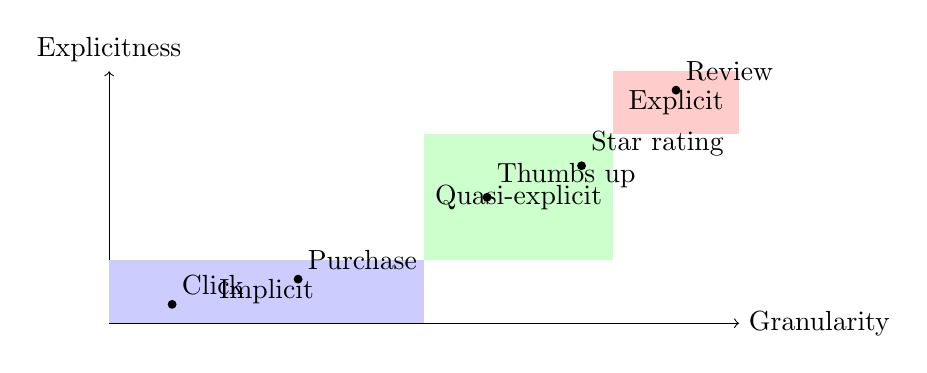
\begin{tikzpicture}[scale=0.8]
    \draw[->] (0,0) -- (10,0) node[right] {Granularity};
    \draw[->] (0,0) -- (0,4) node[above] {Explicitness};

    % Implicit region
    \fill[blue!20] (0,0) rectangle (5,1);
    \node at (2.5,0.5) {Implicit};

    % Quasi-explicit region
    \fill[green!20] (5,1) rectangle (8,3);
    \node at (6.5,2) {Quasi-explicit};

    % Explicit region
    \fill[red!20] (8,3) rectangle (10,4);
    \node at (9,3.5) {Explicit};

    % Example points
    \fill[black] (1,0.3) circle (2pt) node[above right] {Click};
    \fill[black] (3,0.7) circle (2pt) node[above right] {Purchase};
    \fill[black] (6,2) circle (2pt) node[above right] {Thumbs up};
    \fill[black] (7.5,2.5) circle (2pt) node[above right] {Star rating};
    \fill[black] (9,3.7) circle (2pt) node[above right] {Review};
\end{tikzpicture}
\caption{Feedback Granularity Spectrum}
\label{fig:granularity_spectrum}
\end{figure}

\subsubsection{Multimodal Feedback Integration}

Modern systems increasingly combine multiple feedback modalities:
\begin{itemize}
    \item \textbf{Text-visual feedback}: Product images with review text
    \item \textbf{Audio-temporal feedback}: Music listening with skip behaviors
    \item \textbf{Spatial-temporal feedback}: Location-based preferences over time
    \item \textbf{Social-contextual feedback}: Group preferences in social settings
\end{itemize}

\subsubsection{Feedback Reliability Metrics}

Different feedback types have varying reliability characteristics:
\begin{itemize}
    \item \textbf{Internal consistency}: How consistent feedback is within a user
    \item \textbf{External validity}: How well feedback predicts actual behavior
    \item \textbf{Temporal stability}: How consistent feedback is over time
    \item \textbf{Cross-platform consistency}: Feedback agreement across different contexts
\end{itemize}

\subsection{Data Collection Mechanisms and Infrastructure}

\subsubsection{Implicit Feedback Collection}

Implicit feedback collection requires sophisticated tracking infrastructure:
\begin{itemize}
    \item \textbf{Event logging systems}: Real-time capture of user interactions
    \item \textbf{Cookie and session tracking}: Maintaining user identity across sessions
    \item \textbf{Device fingerprinting}: Cross-device user identification
    \item \textbf{Third-party data integration}: Incorporating external behavioral signals
\end{itemize}

\subsubsection{Explicit Feedback Collection}

Explicit feedback requires user interface design and motivation strategies:
\begin{itemize}
    \item \textbf{Rating interfaces}: Intuitive widgets for preference expression
    \item \textbf{Incentive systems}: Gamification and rewards for feedback provision
    \item \textbf{Progressive disclosure}: Multi-step feedback collection to reduce burden
    \item \textbf{Conversational interfaces}: Natural language feedback elicitation
\end{itemize}

\subsubsection{Hybrid Collection Strategies}

Combining collection approaches for comprehensive feedback:
\begin{itemize}
    \item \textbf{Implicit-explicit cascades}: Using implicit signals to trigger explicit feedback requests
    \item \textbf{Multi-touch attribution}: Combining multiple feedback sources for robust signals
    \item \textbf{Adaptive collection}: Dynamically adjusting feedback requests based on user engagement
\end{itemize}

\subsection{Privacy and Ethical Considerations}

\subsubsection{Privacy Implications by Feedback Type}

\begin{table}[h]
\centering
\caption{Privacy and Ethical Dimensions of Feedback Types}
\label{tab:privacy_ethics}
\begin{tabular}{@{}lccc@{}}
\toprule
Dimension & Implicit Feedback & Explicit Feedback & Key Concerns \\
\midrule
Data Sensitivity & Moderate & High & Personal opinion disclosure \\
Collection Transparency & Low & High & User awareness \\
Consent Requirements & Minimal & Explicit & Legal compliance \\
Anonymization Needs & Moderate & High & Identity protection \\
Behavioral Surveillance & High & Low & Privacy erosion \\
Data Minimization & Challenging & Feasible & Storage efficiency \\
User Control & Limited & High & Autonomy preservation \\
Third-party Sharing & Common & Rare & Data brokerage risks \\
\bottomrule
\end{tabular}
\end{table}

\subsubsection{Ethical Challenges}

Feedback collection raises several ethical concerns:
\begin{itemize}
    \item \textbf{Consent and transparency}: Users often unaware of implicit data collection
    \item \textbf{Algorithmic bias amplification}: Feedback patterns reflecting societal biases
    \item \textbf{Manipulation risks}: Systems influencing user behavior through feedback incentives
    \item \textbf{Privacy-utility trade-offs}: Balancing personalization benefits with privacy costs
\end{itemize}

\subsection{Visual Taxonomy and Conceptual Framework}

Figure~\ref{fig:comprehensive_taxonomy} presents our comprehensive taxonomy of feedback types.

\begin{figure}[h]
\centering
\fbox{
\begin{minipage}{0.9\textwidth}
\textbf{Comprehensive Feedback Taxonomy}

\textbf{Main Categories:}
\begin{itemize}
\item \textbf{Implicit Feedback:} User behaviors without conscious effort
  \begin{itemize}
  \item \textit{Micro-level:} Clicks, dwell times, scrolls, hovers
  \item \textit{Meso-level:} Sessions, browsing patterns, purchase sequences
  \item \textit{Macro-level:} Longitudinal behavior, seasonal patterns, life-stage changes
  \end{itemize}
\item \textbf{Explicit Feedback:} Conscious user expressions
  \begin{itemize}
  \item \textit{Quantitative:} Ratings (1-5 stars), numerical scores, Likert scales
  \item \textit{Qualitative:} Reviews, comments, textual descriptions, tags
  \item \textit{Interactive:} Conversations, preference dialogs, custom profiles
  \end{itemize}
\item \textbf{Hybrid Approaches:} Combined implicit and explicit signals
  \begin{itemize}
  \item Multi-modal fusion, confidence-weighted integration, adaptive balancing
  \end{itemize}
\end{itemize}

\textbf{Key Properties by Category:}
\begin{tabular}{@{}lccc@{}}
\toprule
Property & Implicit & Explicit & Hybrid \\
\midrule
Data Abundance & Very High & Low & High \\
Noise Level & High & Low & Medium \\
User Effort & None & High & Medium \\
Temporal Resolution & Real-time & Delayed & Adaptive \\
Interpretability & Low & High & Medium \\
Scalability & High & Moderate & High \\
Privacy Sensitivity & High & Medium & Medium \\
Bias Susceptibility & Behavioral & Selection & Balanced \\
\bottomrule
\end{tabular}
\end{minipage}
}
\caption{Comprehensive taxonomy of implicit and explicit feedback types with hierarchical organization and key properties.}
\label{fig:comprehensive_taxonomy}
\end{figure}

\subsection{Domain-Specific Feedback Characteristics}

Different application domains exhibit unique feedback patterns and requirements:

\subsubsection{E-commerce Feedback Patterns}
\begin{itemize}
    \item High implicit feedback volume from browsing and purchasing
    \item Explicit reviews crucial for trust and explainability
    \item Strong correlation between implicit browsing and explicit purchasing decisions
\end{itemize}

\subsubsection{Entertainment Feedback Dynamics}
\begin{itemize}
    \item Implicit consumption patterns (watch time, skip rates) dominate
    \item Explicit ratings often retrospective and mood-dependent
    \item Social feedback (shares, recommendations) amplifies reach
\end{itemize}

\subsubsection{Social Media Feedback Ecology}
\begin{itemize}
    \item Implicit engagement metrics drive algorithmic ranking
    \item Explicit feedback sparse but highly influential
    \item Network effects create complex feedback cascades
\end{itemize}

This comprehensive taxonomy provides a foundation for understanding the rich landscape of feedback types in recommender systems, enabling more nuanced algorithm design and evaluation approaches.

\section{Learning Paradigms and Modeling Approaches}
\label{sec:learning}

This section provides an extensive review of how implicit and explicit feedback are modeled across classical and modern approaches, including hybrid methods that integrate both types. We cover algorithmic foundations, mathematical formulations, and practical implementation considerations.

\subsection{Classical Approaches}

\subsubsection{Matrix Factorization Fundamentals}

Matrix factorization decomposes user-item interaction matrices into latent factor representations. For explicit feedback, the problem is formulated as:

\begin{equation}
\min_{P,Q} \sum_{(u,i) \in \mathcal{R}} (r_{ui} - p_u^T q_i)^2 + \lambda (\|P\|^2 + \|Q\|^2)
\label{eq:explicit_mf}
\end{equation}

where $r_{ui}$ represents explicit ratings, $p_u$ and $q_i$ are user and item latent factors, and $\lambda$ is a regularization parameter.

For implicit feedback, the formulation changes to handle binary preferences:

\begin{equation}
\min_{P,Q} \sum_{(u,i) \in \mathcal{R}^+} w_{ui} (1 - p_u^T q_i)^2 + \lambda (\|P\|^2 + \|Q\|^2)
\label{eq:implicit_mf}
\end{equation}

where $\mathcal{R}^+$ denotes observed implicit interactions and $w_{ui}$ represents confidence weights.

\subsubsection{Weighted Matrix Factorization (WMF)}

WMF addresses implicit feedback sparsity by treating unobserved interactions as negative signals with varying confidence:

\begin{equation}
\min_{P,Q} \sum_{u,i} c_{ui} (p_{ui} - p_u^T q_i)^2 + \lambda (\|P\|^2 + \|Q\|^2)
\label{eq:wmf}
\end{equation}

where $c_{ui} = \alpha r_{ui}$ for observed interactions and $c_{ui} = 1$ for unobserved ones, with $r_{ui}$ being the implicit feedback strength.

\subsubsection{Bayesian Personalized Ranking (BPR)}

BPR optimizes for ranking rather than rating prediction, using pairwise preferences:

\begin{equation}
\min_{\Theta} -\sum_{(u,i,j) \in D} \ln \sigma(\hat{r}_{ui} - \hat{r}_{uj}) + \lambda_\Theta \|\Theta\|^2
\label{eq:bpr}
\end{equation}

where $D$ contains triples $(u,i,j)$ indicating user $u$ prefers item $i$ over item $j$.

\subsection{Deep Learning Architectures}

\subsubsection{Neural Collaborative Filtering (NCF)}

NCF extends matrix factorization with neural networks:

\begin{equation}
\hat{y}_{ui} = f(p_u, q_i, p_u \odot q_i | \Theta)
\label{eq:ncf}
\end{equation}

where $f(\cdot)$ is a neural network that learns complex interaction patterns from both implicit and explicit feedback.

\subsubsection{Autoencoders for Implicit Feedback}

Denoising autoencoders reconstruct user feedback vectors:

\begin{equation}
\hat{r}_u = f_\theta(f_\phi(r_u + \epsilon))
\label{eq:autoencoder}
\end{equation}

where $\epsilon$ represents noise injection to improve generalization.

\subsubsection{Graph Neural Networks (GNNs)}

GNNs model user-item interactions as graphs:

\begin{equation}
h_u^{(l+1)} = \sigma\left(\sum_{v \in \mathcal{N}(u)} \frac{1}{\sqrt{|\mathcal{N}(u)||\mathcal{N}(v)|}} W^{(l)} h_v^{(l)}\right)
\label{eq:gnn}
\end{equation}

where $\mathcal{N}(u)$ denotes neighbors in the user-item interaction graph.

\subsection{Reinforcement Learning Approaches}

\subsubsection{Markov Decision Processes for Recommendations}

Recommendations are framed as sequential decision-making:

\begin{equation}
\pi^*(s) = \arg\max_\pi \mathbb{E}\left[\sum_{t=0}^\infty \gamma^t r(s_t, a_t) \bigg| s_0 = s, \pi\right]
\label{eq:rl_mdp}
\end{equation}

where states $s$ include user context, actions $a$ are item recommendations, and rewards $r$ come from implicit feedback.

\subsubsection{Contextual Bandits}

Multi-armed bandit approaches balance exploration and exploitation:

\begin{equation}
\mu_{t+1} = \mu_t + \alpha_t (r_t - \mu_t)
\label{eq:bandit_update}
\end{equation}

where $\mu_t$ tracks expected rewards from implicit user responses.

\subsection{Contrastive Learning Paradigms}

\subsubsection{SimCLR for Recommendations}

Contrastive learning maximizes agreement between different views of user-item interactions:

\begin{equation}
\mathcal{L} = -\log \frac{\exp(\text{sim}(z_i, z_j)/\tau)}{\sum_{k=1}^{2N} \mathbb{I}_{[k \neq i]} \exp(\text{sim}(z_i, z_k)/\tau)}
\label{eq:contrastive}
\end{equation}

where $z_i, z_j$ are representations from positive pairs and $\tau$ is temperature.

\subsubsection{Hybrid Contrastive Objectives}

Combining supervised and self-supervised learning:

\begin{equation}
\mathcal{L}_{hybrid} = \mathcal{L}_{supervised} + \lambda \mathcal{L}_{contrastive}
\label{eq:hybrid_contrastive}
\end{equation}

balancing explicit supervision with implicit structure learning.

\subsection{Modern Approaches}

\subsubsection{Deep Learning Models}
Neural networks have revolutionized RS modeling. Autoencoders handle implicit feedback sparsity through reconstruction \cite{sedhain2015autorec}. Convolutional Neural Networks (CNNs) process sequential behaviors \cite{tang2018personalized}. Graph Neural Networks (GNNs) model user-item interactions as graphs \cite{wang2019neural}.

\subsubsection{Reinforcement Learning}
Reinforcement Learning (RL) frames recommendations as sequential decision-making. Implicit feedback serves as rewards, with exploration-exploitation trade-offs \cite{zhao2018recommendations}. Explicit feedback can provide more precise reward signals \cite{chen2019large}.

\subsubsection{Contrastive Learning}
Self-supervised contrastive learning leverages implicit feedback for representation learning. Methods like SimCLR adapt to RS by contrasting user-item interactions \cite{wu2021self}. Hybrid approaches combine contrastive objectives with explicit supervision \cite{xie2022contrastive}.

\subsection{Implicit-to-Explicit Conversions}

Several techniques convert implicit feedback to pseudo-explicit ratings:
\begin{itemize}
    \item \textbf{Ordinal regression}: Maps implicit signals to rating scales \cite{weston2011wsabie}.
    \item \textbf{Confidence weighting}: Assigns confidence scores to implicit preferences \cite{he2016fast}.
    \item \textbf{Generative models}: Uses GANs to synthesize explicit feedback from implicit data \cite{wang2017irgan}.
\end{itemize}

\subsection{Hybrid Models}

Hybrid approaches jointly model both feedback types:
\begin{itemize}
    \item \textbf{Multi-task learning}: Optimizes separate objectives for implicit and explicit feedback \cite{ma2011learning}.
    \item \textbf{Unified frameworks}: Integrates feedback types in shared latent spaces \cite{lian2017cccfnet}.
    \item \textbf{Attention mechanisms}: Weights different feedback sources dynamically \cite{chen2017attentive}.
\end{itemize}

\subsection{Detailed Modeling Techniques}

\subsubsection{Neural Matrix Factorization}

Neural extensions of matrix factorization use multi-layer perceptrons to model non-linear interactions. For implicit feedback, models like NeuMF \cite{he2017neural} learn from binary preferences, achieving state-of-the-art performance on ranking tasks.

\subsubsection{Sequence Modeling}

Recurrent Neural Networks (RNNs) and Transformers capture temporal dependencies in implicit feedback sequences. Models like BERT4Rec \cite{sun2019bert4rec} treat recommendation as a sequence prediction problem.

\subsubsection{Graph-Based Approaches}

Graph Neural Networks model user-item interactions as heterogeneous graphs. Methods like LightGCN \cite{he2020lightgcn} propagate preferences through graph convolutions, effectively handling implicit feedback sparsity.

\subsubsection{Generative Models}

Variational Autoencoders (VAEs) and Generative Adversarial Networks (GANs) generate synthetic feedback. For implicit data, VAEs learn latent representations that reconstruct user behavior patterns.

\subsection{Hybrid Integration Strategies}

\subsubsection{Attention-Based Fusion}

Attention mechanisms dynamically weight feedback sources. For example, in a music recommender, recent explicit ratings might receive higher attention than older implicit plays.

\subsubsection{Multi-Modal Learning}

Combining feedback with content features (e.g., item descriptions) enhances modeling. Vision-language models process explicit reviews alongside implicit clicks.

\subsubsection{Cross-Feedback Translation}

Techniques translate between feedback types. For instance, using LLMs to generate explicit ratings from implicit patterns.

\subsection{Computational Complexity and Scalability}

Implicit feedback models must handle large-scale data. Techniques like negative sampling and distributed training enable scalability. Explicit feedback models are computationally lighter but data-scarce.

\subsection{Evaluation of Modeling Approaches}

Empirical studies show that hybrid models outperform single-type approaches. However, performance gains depend on domain and data quality.

\subsection{Case Studies}

\subsubsection{YouTube Recommendations}

YouTube uses implicit watch time extensively, combined with explicit likes/dislikes. Their system employs deep neural networks for real-time personalization.

\subsubsection{Amazon Product Recommendations}

Amazon integrates purchase history (implicit) with reviews (explicit) using collaborative filtering and content-based methods.

\subsection{Advanced Implementation Considerations}

\subsubsection{Hyperparameter Optimization Strategies}

Effective hyperparameter tuning is crucial for model performance:

\begin{itemize}
    \item \textbf{Grid Search vs. Random Search}: Random search often more efficient for high-dimensional spaces
    \item \textbf{Bayesian Optimization}: Gaussian processes for sample-efficient optimization
    \item \textbf{AutoML Approaches}: Automated machine learning for hyperparameter discovery
    \item \textbf{Domain-Specific Tuning}: Different optimal parameters for implicit vs. explicit feedback
\end{itemize}

\subsubsection{Model Interpretability and Explainability}

Understanding model decisions is increasingly important:

\begin{itemize}
    \item \textbf{Attention Visualization}: Interpreting which feedback sources influence predictions
    \item \textbf{Feature Importance}: Identifying key implicit signals and explicit features
    \item \textbf{Counterfactual Explanations}: Explaining recommendations through "what-if" scenarios
    \item \textbf{User-Centric Explanations}: Translating technical model outputs to user-understandable insights
\end{itemize}

\subsubsection{Online Learning and Adaptation}

Systems must adapt to evolving user preferences:

\begin{itemize}
    \item \textbf{Incremental Learning}: Updating models with new feedback without full retraining
    \item \textbf{Concept Drift Detection}: Identifying when user preferences change significantly
    \item \textbf{Temporal Regularization}: Balancing historical and recent feedback appropriately
    \item \textbf{Context-Aware Updates}: Adapting to changing situational contexts
\end{itemize}

\subsubsection{Computational Resource Management}

Efficient deployment requires careful resource allocation:

\begin{itemize}
    \item \textbf{Model Compression}: Reducing model size for edge deployment
    \item \textbf{Inference Optimization}: Fast prediction serving for real-time recommendations
    \item \textbf{Caching Strategies}: Intelligent caching of user representations and item embeddings
    \item \textbf{Distributed Serving}: Scaling recommendation serving across multiple machines
\end{itemize}

\subsection{Emerging Algorithmic Paradigms}

\subsubsection{Multimodal Recommender Systems}

Integrating multiple data modalities for richer recommendations:

\begin{itemize}
    \item \textbf{Vision-Language Models}: Processing product images with textual reviews
    \item \textbf{Audio-Textual Integration}: Combining music audio features with user listening history
    \item \textbf{Cross-Modal Translation}: Converting between different feedback modalities
    \item \textbf{Multimodal Fusion Architectures}: Attention-based fusion of heterogeneous signals
\end{itemize}

\subsubsection{Causal Inference in Recommendations}

Understanding causal relationships rather than mere correlations:

\begin{itemize}
    \item \textbf{Causal Graphs}: Modeling causal pathways from feedback to user satisfaction
    \item \textbf{Intervention Analysis}: Simulating the effects of different recommendation strategies
    \item \textbf{Counterfactual Reasoning}: Estimating what would have happened under different conditions
    \item \textbf{Bias Mitigation}: Removing spurious correlations through causal methods
\end{itemize}

\subsubsection{Federated and Privacy-Preserving Learning}

Collaborative learning without compromising privacy:

\begin{itemize}
    \item \textbf{Federated Matrix Factorization}: Distributed training across user devices
    \item \textbf{Differential Privacy}: Adding noise to protect individual feedback
    \item \textbf{Secure Multi-Party Computation}: Privacy-preserving collaborative filtering
    \item \textbf{Homomorphic Encryption}: Encrypted computation on sensitive feedback data
\end{itemize}

\subsubsection{Continual and Lifelong Learning}

Adapting to evolving user preferences over time:

\begin{itemize}
    \item \textbf{Catastrophic Forgetting Prevention}: Maintaining old knowledge while learning new patterns
    \item \textbf{Elastic Weight Consolidation}: Protecting important parameters during updates
    \item \textbf{Progressive Neural Networks}: Growing network capacity for new tasks
    \item \textbf{Memory Replay}: Rehearsing past experiences to maintain performance
\end{itemize}

\subsection{Open Challenges in Modeling}

\begin{itemize}
    \item Handling feedback conflicts (e.g., clicking but not purchasing).
    \item Modeling long-term vs. short-term preferences.
    \item Incorporating user context and demographics.
\end{itemize}

\section{Evaluation Methodologies}
\label{sec:evaluation}

Evaluating recommender systems requires metrics that account for feedback characteristics and potential biases. The choice of evaluation methodology fundamentally depends on the feedback type used, with implicit and explicit feedback requiring different approaches and interpretations.

\subsection{Standard Metrics}

\subsubsection{Ranking Metrics}
Precision@K, Recall@K, Mean Average Precision (MAP), and Normalized Discounted Cumulative Gain (NDCG) assess recommendation quality. These metrics behave differently under implicit vs. explicit feedback:

\begin{itemize}
    \item \textbf{Implicit feedback} often uses binary relevance (clicked/not clicked), favoring ranking accuracy over absolute preference strength.
    \item \textbf{Explicit feedback} incorporates preference strength, allowing for more nuanced evaluation of recommendation quality.
    \item \textbf{Hybrid approaches} require careful calibration to balance ranking and rating prediction objectives.
\end{itemize}

The mathematical formulations reveal important differences:

\begin{equation}
\text{Precision@K} = \frac{|\{i \in \text{top-K} \cap \text{relevant}\}|}{K}
\label{eq:precision_k}
\end{equation}

\begin{equation}
\text{NDCG@K} = \frac{1}{|U|} \sum_{u \in U} \frac{\sum_{i=1}^K \frac{rel_{u,i}}{log_2(i+1)}}{\sum_{i=1}^{|REL_u|} \frac{1}{log_2(i+1)}}
\label{eq:ndcg_k}
\end{equation}

where $rel_{u,i}$ represents relevance scores that differ significantly between implicit (binary) and explicit (graded) feedback.

\subsubsection{Rating Prediction Metrics}
Root Mean Square Error (RMSE) and Mean Absolute Error (MAE) evaluate explicit rating predictions:

\begin{equation}
\text{RMSE} = \sqrt{\frac{1}{|R|} \sum_{(u,i) \in R} (\hat{r}_{ui} - r_{ui})^2}
\label{eq:rmse}
\end{equation}

\begin{equation}
\text{MAE} = \frac{1}{|R|} \sum_{(u,i) \in R} |\hat{r}_{ui} - r_{ui}|
\label{eq:mae}
\end{equation}

These metrics are less applicable to implicit feedback, which lacks ground-truth ratings, necessitating alternative evaluation approaches.

\subsubsection{Area Under the Curve (AUC) Metrics}
For implicit feedback evaluation, AUC-based metrics provide robust ranking assessment:

\begin{equation}
\text{AUC} = \frac{1}{|U|} \sum_{u \in U} \frac{1}{|I_u^+||I_u^-|} \sum_{i^+ \in I_u^+} \sum_{i^- \in I_u^-} \mathbb{I}(\hat{r}_{ui^+} > \hat{r}_{ui^-})
\label{eq:auc}
\end{equation}

where $I_u^+$ and $I_u^-$ represent positive and negative feedback items for user $u$.

\subsection{Evaluation Biases and Challenges}

\subsubsection{Dataset Biases}
Public datasets exhibit various biases that affect evaluation reliability:

\begin{table}[h]
\centering
\caption{Evaluation Biases in Different Feedback Types}
\label{tab:evaluation_biases}
\begin{tabular}{@{}lccc@{}}
\toprule
Bias Type & Implicit Feedback & Explicit Feedback & Mitigation Strategies \\
\midrule
Popularity Bias & High (rich-get-richer) & Moderate & Inverse propensity scoring \\
Position Bias & Very High & Moderate & Position debiasing, randomization \\
Selection Bias & Low & Very High & Inverse propensity weighting \\
Confirmation Bias & Moderate & High & Counterfactual evaluation \\
Temporal Bias & High & Moderate & Time-aware validation \\
Demographic Bias & Moderate & High & Fairness-aware evaluation \\
\bottomrule
\end{tabular}
\end{table}

\subsubsection{User Behavior Interpretations}
Implicit feedback interpretations can be misleading:

\begin{itemize}
    \item \textbf{Engagement vs. Interest}: Long watch times may indicate engagement or involuntary attention (e.g., background TV)
    \item \textbf{Contextual Influences}: Clicks may result from curiosity, social pressure, or algorithmic manipulation
    \item \textbf{Behavioral Variability}: User interaction patterns vary significantly across demographics and contexts
    \item \textbf{False Negatives}: Lack of interaction doesn't necessarily indicate lack of interest
\end{itemize}

Explicit feedback, while clearer, has its own interpretation challenges:

\begin{itemize}
    \item \textbf{Mood-Dependent Ratings}: Emotional state influences rating consistency
    \item \textbf{Social Desirability Bias}: Users provide socially acceptable rather than genuine opinions
    \item \textbf{Scale Interpretation Variance}: Different users interpret rating scales differently
    \item \textbf{Recency Effects}: Recent experiences disproportionately influence feedback
\end{itemize}

\subsection{Advanced Evaluation Frameworks}

\subsubsection{Novelty and Diversity Metrics}

Beyond accuracy, diversity and novelty are crucial for user satisfaction:

\begin{equation}
\text{Novelty} = -\log_2(\text{popularity}(i))
\label{eq:novelty}
\end{equation}

\begin{equation}
\text{Diversity} = 1 - \frac{\sum_{i,j \in L} s(i,j)}{|L|(|L|-1)}
\label{eq:diversity}
\end{equation}

where $s(i,j)$ measures similarity between recommended items and $L$ is the recommendation list.

\subsubsection{Serendipity Metrics}

Measuring unexpected relevant recommendations:

\begin{equation}
\text{Serendipity} = \frac{1}{|U|} \sum_u \frac{|\{i \in L_u | rel(u,i) \land unexpected(u,i)\}|}{|L_u|}
\label{eq:serendipity}
\end{equation}

\subsubsection{Coverage Metrics}

Assessing catalog utilization:

\begin{equation}
\text{Catalog Coverage} = \frac{|\bigcup_u L_u|}{|\mathcal{I}|}
\label{eq:coverage}
\end{equation}

\begin{equation}
\text{User Coverage} = \frac{|\{u | |L_u| > 0\}|}{|U|}
\label{eq:user_coverage}
\end{equation}

\subsection{User-Centric Evaluation Methods}

\subsubsection{A/B Testing and Online Evaluation}

Real-world performance assessment through controlled experiments:

\begin{itemize}
    \item \textbf{Interleaving Methods}: Comparing ranking algorithms by interleaving recommendations
    \item \textbf{Multi-Armed Bandit Evaluation}: Online learning-based evaluation protocols
    \item \textbf{Counterfactual Evaluation}: Estimating performance under different conditions
\end{itemize}

\subsubsection{User Studies and Surveys}

Qualitative assessment of user experience:

\begin{itemize}
    \item \textbf{Satisfaction Surveys}: Measuring perceived recommendation quality
    \item \textbf{Trust Assessments}: Evaluating system credibility and transparency
    \item \textbf{Behavioral Metrics}: Task completion rates and engagement patterns
    \item \textbf{Longitudinal Studies}: Tracking user behavior over extended periods
\end{itemize}

\subsubsection{Eye-Tracking and Physiological Measures}

Advanced user response measurement:

\begin{itemize}
    \item \textbf{Fixation Duration}: Measuring attention to recommended items
    \item \textbf{Pupil Dilation}: Indicating cognitive load and interest intensity
    \item \textbf{Heart Rate Variability}: Assessing emotional responses to recommendations
\end{itemize}

\subsection{Bias Mitigation in Evaluation}

\subsubsection{Debiasing Techniques}

Addressing evaluation biases through statistical corrections:

\begin{itemize}
    \item \textbf{Inverse Propensity Scoring}: Correcting for selection biases in explicit feedback
    \item \textbf{Position Bias Debiasing}: Accounting for presentation order effects
    \item \textbf{Popularity Bias Correction}: Balancing evaluation across item popularity levels
    \item \textbf{Temporal Debiasing}: Handling temporal distribution shifts in feedback
\end{itemize}

\subsubsection{Fairness-Aware Evaluation}

Ensuring equitable performance across user groups:

\begin{equation}
\text{Demographic Parity} = \max_g \left| \frac{|\{u \in g | \text{satisfied}(u)\}|}{|g|} - \frac{|\{u \notin g | \text{satisfied}(u)\}|}{|U \setminus g|} \right|
\label{eq:demographic_parity}
\end{equation}

\subsection{Dataset Construction and Benchmarking}

\subsubsection{Synthetic Dataset Generation}

Creating controlled evaluation environments:

\begin{itemize}
    \item \textbf{Simulation-Based Datasets}: Generating feedback based on known user preferences
    \item \textbf{Counterfactual Datasets}: Creating "what-if" scenarios for causal evaluation
    \item \textbf{Multi-Behavior Datasets}: Capturing diverse feedback types simultaneously
\end{itemize}

\subsubsection{Cross-Domain Evaluation}

Assessing generalizability across different contexts:

\begin{itemize}
    \item \textbf{Domain Adaptation Metrics}: Measuring performance transfer between domains
    \item \textbf{Out-of-Distribution Evaluation}: Testing robustness to novel scenarios
    \item \textbf{Meta-Evaluation}: Evaluating evaluation metrics themselves
\end{itemize}

\subsection{Statistical Rigor and Reproducibility}

\subsubsection{Confidence Intervals and Significance Testing}

Ensuring reliable performance comparisons:

\begin{equation}
\text{Confidence Interval} = \bar{x} \pm z \cdot \frac{\sigma}{\sqrt{n}}
\label{eq:confidence_interval}
\end{equation}

\subsubsection{Reproducibility Challenges}

Addressing evaluation variability:

\begin{itemize}
    \item \textbf{Algorithmic Randomness}: Controlling stochastic elements in model training
    \item \textbf{Dataset Splits}: Ensuring consistent train/test/validation partitions
    \item \textbf{Hyperparameter Sensitivity}: Reporting performance across parameter ranges
    \item \textbf{Computational Reproducibility}: Managing hardware and software dependencies
\end{itemize}

\subsection{Domain-Specific Evaluation Considerations}

\subsubsection{E-commerce Evaluation}

Focusing on conversion and revenue metrics:

\begin{itemize}
    \item \textbf{Conversion Rate}: Percentage of recommendations leading to purchases
    \item \textbf{Revenue per User}: Economic impact of recommendation strategies
    \item \textbf{Cart Completion Rate}: Effectiveness in reducing abandonment
    \item \textbf{Cross-Sell Performance}: Success in suggesting complementary products
\end{itemize}

\subsubsection{Content Streaming Evaluation}

Emphasizing engagement and retention:

\begin{itemize}
    \item \textbf{Watch Time}: Total engagement duration with recommended content
    \item \textbf{Completion Rate}: Percentage of content consumed to completion
    \item \textbf{Skip Rate}: Negative feedback through content abandonment
    \item \textbf{Return Visits}: Long-term user retention and loyalty
\end{itemize}

\subsubsection{Social Media Evaluation}

Measuring network and information effects:

\begin{itemize}
    \item \textbf{Viral Coefficient}: Amplification of content through social sharing
    \item \textbf{Engagement Rate}: Likes, comments, and shares per recommendation
    \item \textbf{Information Diversity}: Balance between personalized and diverse content
    \item \textbf{Polarization Metrics}: Assessing filter bubble effects
\end{itemize}

\subsection{Temporal and Dynamic Evaluation}

\subsubsection{Concept Drift Detection}

Monitoring performance stability over time:

\begin{equation}
\text{Drift Score} = \frac{1}{T} \sum_{t=1}^T |\mu_{t} - \mu_{t-1}|
\label{eq:drift_score}
\end{equation}

where $\mu_t$ represents performance metrics at time $t$.

\subsubsection{Adaptive Evaluation Protocols}

Dynamic assessment methods for evolving systems:

\begin{itemize}
    \item \textbf{Online Learning Evaluation}: Continuous performance monitoring
    \item \textbf{Contextual Evaluation}: Performance assessment under different conditions
    \item \textbf{Multi-Horizon Evaluation}: Short-term vs. long-term impact assessment
\end{itemize}

\subsection{Future Evaluation Directions}

Emerging evaluation paradigms include:

\begin{itemize}
    \item \textbf{Causal Evaluation}: Understanding causal relationships between recommendations and outcomes
    \item \textbf{Multimodal Evaluation}: Assessing performance across different feedback modalities
    \item \textbf{Human-AI Collaborative Evaluation}: Combining automated metrics with human judgment
    \item \textbf{Sustainable Evaluation}: Measuring environmental and social impact of recommendation systems
\end{itemize}

This comprehensive evaluation framework ensures that recommender systems are assessed appropriately for their feedback characteristics, providing reliable and meaningful performance comparisons across different approaches and domains.

\section{Applications and Domains}
\label{sec:applications}

Implicit and explicit feedback find applications across diverse domains, with feedback types influencing personalization strategies, user experience, and business outcomes. This section provides comprehensive analysis of how different feedback modalities shape recommendation systems in various industries and use cases.

\subsection{E-commerce and Retail}

\subsubsection{Product Recommendation Systems}

E-commerce platforms leverage complex feedback ecosystems:

\begin{itemize}
    \item \textbf{Implicit Feedback Sources}: Clickstreams, browsing patterns, cart additions, purchase sequences, search queries, and time spent on product pages
    \item \textbf{Explicit Feedback Sources}: Product ratings, detailed reviews, wishlists, and return/refund feedback
    \item \textbf{Hybrid Integration}: Combining browsing intent with review validation for purchase prediction
\end{itemize}

Key challenges include:
\begin{itemize}
    \item \textbf{Abandonment Prediction}: Using implicit signals to identify at-risk shopping carts
    \item \textbf{Cross-Sell Optimization}: Recommending complementary products based on purchase patterns
    \item \textbf{Personalized Pricing}: Dynamic pricing based on user engagement and purchase history
    \item \textbf{Inventory Management}: Demand forecasting using implicit browsing trends
\end{itemize}

\subsubsection{Case Studies}

\textbf{Amazon's Recommendation Engine}:
\begin{itemize}
    \item Processes billions of implicit interactions daily
    \item "Customers who bought this also bought" uses collaborative filtering on purchase data
    \item "Frequently bought together" leverages co-purchase patterns
    \item Explicit reviews influence product ranking and visibility
    \item Hybrid models achieve 35\% of all purchases through recommendations
\end{itemize}

\textbf{Alibaba's Taobao Platform}:
\begin{itemize}
    \item Real-time implicit feedback processing for flash sales
    \item Social commerce integration with explicit friend recommendations
    \item Mobile-optimized implicit feedback (touch gestures, scroll patterns)
    \item Cross-border recommendation challenges with cultural feedback differences
\end{itemize}

\subsubsection{Performance Metrics}

E-commerce success metrics include:
\begin{itemize}
    \item \textbf{Conversion Rate}: Click-to-purchase ratios (typically 2-5\%)
    \item \textbf{Average Order Value}: Revenue impact of recommendations
    \item \textbf{Cart Completion Rate}: Reduction in abandonment through personalized suggestions
    \item \textbf{Return Rate}: Quality of recommendations measured by post-purchase satisfaction
\end{itemize}

\subsection{Content Streaming and Entertainment}

\subsubsection{Video Streaming Platforms}

Netflix, YouTube, and similar platforms rely heavily on implicit feedback:

\begin{itemize}
    \item \textbf{Implicit Signals}: Watch time, completion rates, skip behavior, pause patterns, rewind/fast-forward actions
    \item \textbf{Explicit Signals}: Thumbs up/down, ratings, reviews, playlist creation
    \item \textbf{Contextual Factors}: Time of day, device type, binge-watching patterns
\end{itemize}

Advanced applications include:
\begin{itemize}
    \item \textbf{Content Discovery}: Genre exploration based on viewing patterns
    \item \textbf{Binge Prediction}: Anticipating multi-episode consumption
    \item \textbf{Ad Insertion}: Optimal placement based on engagement patterns
    \item \textbf{Content Creation}: Using feedback to guide production decisions
\end{itemize}

\subsubsection{Music Streaming Services}

Spotify and Apple Music optimize for user engagement:

\begin{itemize}
    \item \textbf{Implicit Feedback}: Play counts, skip rates, playlist additions, repeat listens, share actions
    \item \textbf{Explicit Feedback}: Song ratings, playlist curation, artist follows, concert ticket purchases
    \item \textbf{Temporal Patterns}: Daily routines, mood-based listening, social sharing
\end{itemize}

Key innovations:
\begin{itemize}
    \item \textbf{Discover Weekly}: Algorithmic playlist generation from listening history
    \item \textbf{Blend Playlists}: Social music discovery through shared listening patterns
    \item \textbf{Mood Detection}: Inferring emotional state from music selection patterns
    \item \textbf{Live Performance Prediction}: Concert recommendations based on artist engagement
\end{itemize}

\subsubsection{Case Study: Netflix Recommendation System}

\begin{itemize}
    \item \textbf{Data Scale}: Processes 500+ billion user interactions daily
    \item \textbf{Implicit Dominance}: 95\% of viewing decisions based on implicit feedback
    \item \textbf{Personalized Thumbnails}: A/B testing different artwork based on user preferences
    \item \textbf{Row Personalization}: Dynamic content organization based on viewing history
    \item \textbf{Impact}: Accounts for 80\% of viewing time, prevents churn through engagement
\end{itemize}

\subsection{News and Content Platforms}

\subsubsection{News Recommendation Challenges}

News platforms balance timeliness with quality:

\begin{itemize}
    \item \textbf{Implicit Feedback}: Click-through rates, dwell time, scroll depth, sharing actions
    \item \textbf{Explicit Feedback}: Article ratings, topic preferences, follow actions, report buttons
    \item \textbf{Quality Signals}: Time spent reading, return visits, bookmarking behavior
\end{itemize}

Critical considerations:
\begin{itemize}
    \item \textbf{Filter Bubble Mitigation}: Balancing personalization with diversity
    \item \textbf{Fake News Detection}: Using engagement patterns to identify misinformation
    \item \textbf{Breakthrough Discovery}: Introducing users to new topics and perspectives
    \item \textbf{Real-time Adaptation}: Responding to breaking news and trending topics
\end{itemize}

\subsubsection{Social News Platforms}

Reddit and similar platforms use community feedback:

\begin{itemize}
    \item \textbf{Implicit Signals}: Upvote timing, comment engagement, subreddit subscriptions
    \item \textbf{Explicit Signals}: Direct feedback, moderator actions, community guidelines
    \item \textbf{Social Dynamics}: Influence propagation through social networks
\end{itemize}

\subsection{Social Media and Networking}

\subsubsection{Content Ranking Algorithms}

Facebook, Twitter, and Instagram optimize for engagement:

\begin{itemize}
    \item \textbf{Implicit Feedback}: Likes, shares, comments, view duration, profile visits
    \item \textbf{Explicit Feedback}: Follow/unfollow actions, content reports, privacy settings
    \item \textbf{Network Effects}: Social graph analysis and influence propagation
\end{itemize}

Key applications:
\begin{itemize}
    \item \textbf{Feed Personalization}: Algorithmic content ranking for individual users
    \item \textbf{Ad Targeting}: Precise audience segmentation based on behavioral patterns
    \item \textbf{Community Detection}: Identifying interest groups and social clusters
    \item \textbf{Influence Maximization}: Optimizing content spread through social networks
\end{itemize}

\subsubsection{Case Study: Twitter's Algorithm}

\begin{itemize}
    \item \textbf{Multi-Objective Optimization}: Balancing engagement, relevance, and recency
    \item \textbf{Implicit Signals}: Retweet patterns, quote tweet behavior, thread engagement
    \item \textbf{Real-time Processing}: Adapting to trending topics and breaking news
    \item \textbf{Conversation Health}: Promoting constructive dialogue through feedback analysis
\end{itemize}

\subsection{Emerging Domains and Applications}

\subsubsection{Educational Platforms}

Learning management systems use feedback for personalization:

\begin{itemize}
    \item \textbf{Implicit Feedback}: Time spent on materials, quiz attempt patterns, navigation sequences
    \item \textbf{Explicit Feedback}: Course ratings, assignment feedback, learning goal declarations
    \item \textbf{Adaptive Learning}: Personalizing content difficulty and pacing based on engagement
\end{itemize}

\subsubsection{Health and Fitness Applications}

Wellness apps optimize for behavior change:

\begin{itemize}
    \item \textbf{Implicit Feedback}: Workout completion, step counts, sleep patterns, app usage frequency
    \item \textbf{Explicit Feedback}: Goal setting, satisfaction surveys, pain level reporting
    \item \textbf{Motivation Systems}: Using engagement patterns to provide timely encouragement
\end{itemize}

\subsubsection{Professional Networking}

LinkedIn and similar platforms focus on career development:

\begin{itemize}
    \item \textbf{Implicit Feedback}: Profile view patterns, connection requests, content engagement
    \item \textbf{Explicit Feedback}: Endorsements, recommendations, skill assessments
    \item \textbf{Career Path Prediction}: Using interaction patterns to suggest professional development
\end{itemize}

\subsubsection{Gaming and Interactive Entertainment}

Game platforms personalize player experiences:

\begin{itemize}
    \item \textbf{Implicit Feedback}: Play time, level completion, in-game purchases, social interactions
    \item \textbf{Explicit Feedback}: Game ratings, review comments, friend recommendations
    \item \textbf{Dynamic Difficulty}: Adjusting challenge levels based on player skill patterns
\end{itemize}

\subsection{Domain-Specific Feedback Characteristics}

\subsubsection{Feedback Abundance and Quality}

Different domains exhibit varying feedback landscapes:

\begin{table}[h]
\centering
\caption{Feedback Characteristics Across Domains}
\label{tab:domain_feedback}
\begin{tabular}{@{}lcccc@{}}
\toprule
Domain & Implicit Volume & Explicit Quality & Real-time Needs & Privacy Sensitivity \\
\midrule
E-commerce & Very High & High & Medium & Medium \\
Video Streaming & Extremely High & Medium & High & Low \\
Music Streaming & High & Medium & High & Low \\
News & High & Low & Very High & Medium \\
Social Media & Very High & Low & Very High & High \\
Education & Medium & High & Low & High \\
Health/Fitness & High & Medium & Medium & Very High \\
Professional & Medium & High & Low & High \\
Gaming & High & Medium & High & Medium \\
\bottomrule
\end{tabular}
\end{table}

\subsubsection{Cross-Domain Feedback Transfer}

Understanding feedback patterns across domains enables transfer learning:

\begin{itemize}
    \item \textbf{Music to Video}: Audio preferences predicting visual content interests
    \item \textbf{Shopping to Entertainment}: Purchase patterns informing content recommendations
    \item \textbf{Social to Professional}: Network behavior patterns in career contexts
    \item \textbf{Educational to Gaming}: Learning patterns informing game personalization
\end{itemize}

\subsection{Industry Best Practices and Implementation}

\subsubsection{Data Pipeline Architecture}

Successful implementations require robust infrastructure:

\begin{itemize}
    \item \textbf{Real-time Processing}: Streaming analytics for immediate feedback incorporation
    \item \textbf{Scalable Storage}: Distributed databases handling massive feedback volumes
    \item \textbf{Privacy Compliance}: GDPR/CCPA-compliant data handling and user consent management
    \item \textbf{A/B Testing Frameworks}: Continuous experimentation and performance monitoring
\end{itemize}

\subsubsection{Model Deployment and Monitoring}

Production systems require careful management:

\begin{itemize}
    \item \textbf{Online Learning}: Continuous model updates with new feedback
    \item \textbf{Performance Monitoring}: Real-time tracking of recommendation quality metrics
    \item \textbf{Fallback Strategies}: Graceful degradation when feedback signals are weak
    \item \textbf{Bias Detection}: Ongoing monitoring for unfair or discriminatory patterns
\end{itemize}

\subsubsection{User Experience Optimization}

Feedback integration affects user satisfaction:

\begin{itemize}
    \item \textbf{Seamless Integration}: Implicit feedback collection without disrupting user flow
    \item \textbf{Transparency}: Clear communication about how feedback influences recommendations
    \item \textbf{Control Mechanisms}: User options to adjust feedback sensitivity and preferences
    \item \textbf{Privacy Controls}: Granular permissions for different feedback types
\end{itemize}

\subsection{Impact on Business Outcomes}

\subsubsection{Quantitative Benefits}

Successful feedback integration drives measurable improvements:

\begin{itemize}
    \item \textbf{Revenue Impact}: 15-35\% increase in conversion rates through personalized recommendations
    \item \textbf{User Engagement}: 20-50\% improvement in session duration and return visits
    \item \textbf{Customer Satisfaction}: Higher NPS scores through relevant personalization
    \item \textbf{Operational Efficiency}: Reduced support costs through proactive recommendations
\end{itemize}

\subsubsection{Qualitative Benefits}

Beyond metrics, feedback systems provide strategic advantages:

\begin{itemize}
    \item \textbf{Competitive Differentiation}: Superior personalization as a market advantage
    \item \textbf{Customer Loyalty}: Building long-term relationships through understanding
    \item \textbf{Innovation Opportunities}: Data-driven insights for product development
    \item \textbf{Risk Mitigation}: Early detection of user dissatisfaction and churn signals
\end{itemize}

\subsection{Future Domain Evolution}

Emerging trends will reshape feedback utilization:

\begin{itemize}
    \item \textbf{Metaverse Integration}: Spatial and embodied feedback in virtual environments
    \item \textbf{IoT Ecosystem}: Connected device feedback for holistic user understanding
    \item \textbf{Brain-Computer Interfaces}: Direct neural feedback for ultimate personalization
    \item \textbf{Quantum Computing}: Massive-scale feedback processing for unprecedented accuracy
\end{itemize}

This comprehensive analysis demonstrates how feedback types fundamentally shape recommendation system design and outcomes across diverse application domains, with each domain requiring tailored approaches to maximize effectiveness and user satisfaction.

\section{Challenges and Future Directions}
\label{sec:challenges}

Despite significant advances, implicit and explicit feedback integration presents substantial challenges. This section examines current limitations and emerging research directions that will shape the next generation of recommendation systems.

\subsection{Technical Challenges}

\subsubsection{Data Quality and Noise Issues}

Feedback signals are inherently noisy and require sophisticated processing:

\begin{itemize}
    \item \textbf{Implicit Feedback Noise}: User actions may not reflect true preferences (accidental clicks, external influences)
    \item \textbf{Explicit Feedback Bias}: Self-selection bias in rating systems, where only highly satisfied/dissatisfied users provide feedback
    \item \textbf{Contextual Interference}: Environmental factors affecting feedback interpretation (time pressure, device limitations)
    \item \textbf{Adversarial Manipulation}: Malicious users attempting to game recommendation algorithms
\end{itemize}

Mathematical formulation of noise in implicit feedback:
\begin{equation}
y_{ui} = f(p_{ui}) + \epsilon_{ui} + \eta_{ui}
\end{equation}
where $y_{ui}$ is observed feedback, $f(p_{ui})$ is true preference, $\epsilon_{ui}$ is random noise, and $\eta_{ui}$ is systematic bias.

\subsubsection{Sparsity and Cold-Start Problems}

New users and items lack sufficient feedback history:

\begin{itemize}
    \item \textbf{User Cold-Start}: New users with minimal interaction history
    \item \textbf{Item Cold-Start}: New items without feedback data
    \item \textbf{System Cold-Start}: Launching new recommendation systems from scratch
    \item \textbf{Domain Cold-Start}: Applying trained models to new domains
\end{itemize}

Hybrid approaches address sparsity through:
\begin{itemize}
    \item \textbf{Multi-Source Integration}: Combining feedback types to reduce sparsity
    \item \textbf{Transfer Learning}: Leveraging knowledge from related domains
    \item \textbf{Active Learning}: Strategically collecting feedback to maximize information gain
    \item \textbf{Zero-Shot Learning}: Making recommendations without direct feedback history
\end{itemize}

\subsubsection{Scalability and Real-Time Processing}

Large-scale systems face computational challenges:

\begin{itemize}
    \item \textbf{Data Volume}: Processing billions of feedback interactions daily
    \item \textbf{Model Complexity}: Training deep learning models on massive datasets
    \item \textbf{Real-Time Latency}: Sub-second response times for user interactions
    \item \textbf{Distributed Computing}: Coordinating feedback processing across global data centers
\end{itemize}

Optimization techniques include:
\begin{itemize}
    \item \textbf{Approximate Methods}: Using sampling and sketching for large-scale matrix factorization
    \item \textbf{Streaming Algorithms}: Online learning approaches for continuous feedback streams
    \item \textbf{Federated Learning}: Distributed training while preserving user privacy
    \item \textbf{Edge Computing}: Processing feedback closer to users for reduced latency
\end{itemize}

\subsection{Ethical and Societal Challenges}

\subsubsection{Privacy and Data Protection}

Feedback collection raises significant privacy concerns:

\begin{itemize}
    \item \textbf{Implicit Data Sensitivity}: Tracking user behavior without explicit consent
    \item \textbf{Data Minimization}: Collecting only necessary feedback while maintaining effectiveness
    \item \textbf{User Consent}: Transparent opt-in mechanisms for feedback collection
    \item \textbf{Data Ownership}: Users' rights over their feedback data
\end{itemize}

Privacy-preserving techniques:
\begin{itemize}
    \item \textbf{Differential Privacy}: Adding noise to protect individual privacy
    \item \textbf{Federated Learning}: Training models without centralizing user data
    \item \textbf{Local Differential Privacy}: Privacy protection at the device level
    \item \textbf{Homomorphic Encryption}: Computing on encrypted feedback data
\end{itemize}

\subsubsection{Fairness and Bias Mitigation}

Recommendation systems can perpetuate societal biases:

\begin{itemize}
    \item \textbf{Representation Bias}: Under-representation of minority groups in training data
    \item \textbf{Popularity Bias}: Over-recommending popular items, creating rich-get-richer effects
    \item \textbf{Position Bias}: Users' tendency to interact with highly-ranked items
    \item \textbf{Selection Bias}: Non-random feedback collection leading to skewed distributions
\end{itemize}

Fairness-aware approaches:
\begin{itemize}
    \item \textbf{Debiasing Algorithms}: Correcting for known biases in feedback data
    \item \textbf{Diverse Recommendations}: Promoting variety and serendipity
    \item \textbf{Group Fairness}: Ensuring equitable outcomes across demographic groups
    \item \textbf{Individual Fairness}: Treating similar users similarly
\end{itemize}

\subsubsection{Filter Bubbles and Echo Chambers}

Personalization can limit exposure to diverse content:

\begin{itemize}
    \item \textbf{Homophily Effects}: Users increasingly exposed to similar viewpoints
    \item \textbf{Polarization Risks}: Reinforcement of extreme opinions through feedback loops
    \item \textbf{Discovery Reduction}: Decreased exposure to novel or challenging content
    \item \textbf{Social Fragmentation}: Reduced common ground in public discourse
\end{itemize}

Mitigation strategies:
\begin{itemize}
    \item \textbf{Diversity Objectives}: Explicitly optimizing for content variety
    \item \textbf{Serendipity Injection}: Introducing unexpected but relevant recommendations
    \item \textbf{Cross-Cutting Exposure}: Balancing personalization with broad exploration
    \item \textbf{User Control}: Allowing users to adjust personalization intensity
\end{itemize}

\subsection{Explainability and Trust}

\subsubsection{Black-Box Model Transparency}

Complex models lack interpretability:

\begin{itemize}
    \item \textbf{Deep Learning Opacity}: Neural networks as uninterpretable black boxes
    \item \textbf{Hybrid Model Complexity}: Combining multiple feedback types increases opacity
    \item \textbf{Real-Time Explanations}: Providing immediate rationale for recommendations
    \item \textbf{User Comprehension}: Ensuring explanations are understandable to non-experts
\end{itemize}

Explainability techniques:
\begin{itemize}
    \item \textbf{Post-Hoc Explanations}: Interpreting model decisions after prediction
    \item \textbf{Transparent Models}: Using inherently interpretable algorithms
    \item \textbf{Local Explanations}: Explaining individual recommendations
    \item \textbf{Global Explanations}: Understanding overall model behavior
\end{itemize}

\subsubsection{User Trust and Adoption}

Building confidence in recommendation systems:

\begin{itemize}
    \item \textbf{Accuracy-Explainability Trade-off}: More accurate models often less interpretable
    \item \textbf{User Agency}: Providing control over recommendation processes
    \item \textbf{Error Recovery}: Handling and learning from incorrect recommendations
    \item \textbf{Long-term Trust}: Maintaining reliability over extended interactions
\end{itemize}

\subsection{Research Gaps and Opportunities}

\subsubsection{Theoretical Foundations}

Fundamental understanding remains incomplete:

\begin{itemize}
    \item \textbf{Feedback Theory}: Comprehensive theory of implicit vs. explicit feedback
    \item \textbf{Preference Modeling}: Mathematical models of user preference formation
    \item \textbf{Feedback Dynamics}: How feedback evolves over time and context
    \item \textbf{Causal Inference}: Understanding causal relationships in feedback loops
\end{itemize}

\subsubsection{Methodological Advances}

New approaches are needed for emerging challenges:

\begin{itemize}
    \item \textbf{Multimodal Feedback}: Integrating text, images, audio, and sensor data
    \item \textbf{Temporal Modeling}: Capturing evolving preferences over time
    \item \textbf{Social Feedback}: Leveraging social network influences
    \item \textbf{Cross-Domain Transfer}: Applying knowledge across different domains
\end{itemize}

\subsubsection{Evaluation Frameworks}

Better assessment methodologies required:

\begin{itemize}
    \item \textbf{Offline-Online Evaluation}: Bridging simulation and real-world performance
    \item \textbf{User-Centric Metrics}: Beyond accuracy to satisfaction and utility
    \item \textbf{Long-Term Effects}: Measuring sustained impact on user behavior
    \item \textbf{A/B Testing at Scale}: Rigorous experimentation in production systems
\end{itemize}

\subsection{Future Research Directions}

\subsubsection{Emerging Technologies and Paradigms}

New technologies will transform feedback utilization:

\begin{itemize}
    \item \textbf{Brain-Computer Interfaces}: Direct neural feedback for ultimate personalization
    \item \textbf{Extended Reality}: Spatial and embodied feedback in AR/VR environments
    \item \textbf{Quantum Computing}: Massive-scale optimization for recommendation problems
    \item \textbf{Edge AI}: On-device processing for privacy-preserving recommendations
\end{itemize}

\subsubsection{Interdisciplinary Integration}

Cross-disciplinary approaches will drive innovation:

\begin{itemize}
    \item \textbf{Cognitive Science}: Understanding human decision-making processes
    \item \textbf{Social Psychology}: Modeling social influence and group dynamics
    \item \textbf{Economics}: Incentive design for feedback collection and quality
    \item \textbf{Human-Computer Interaction}: Designing intuitive feedback interfaces
\end{itemize}

\subsubsection{Sustainable and Responsible AI}

Long-term societal impact considerations:

\begin{itemize}
    \item \textbf{Energy-Efficient Computing}: Reducing environmental impact of large-scale systems
    \item \textbf{Digital Well-being}: Balancing personalization with mental health
    \item \textbf{Democratic Access}: Ensuring recommendation benefits reach all societal groups
    \item \textbf{Regulatory Compliance}: Adapting to evolving privacy and fairness regulations
\end{itemize}

\subsection{Implementation Challenges}

\subsubsection{System Architecture Evolution}

Future systems will require new architectural paradigms:

\begin{itemize}
    \item \textbf{Microservices Architecture}: Modular feedback processing components
    \item \textbf{Event-Driven Systems}: Real-time feedback stream processing
    \item \textbf{Serverless Computing}: Elastic scaling for variable feedback loads
    \item \textbf{Blockchain Integration}: Decentralized feedback verification and ownership
\end{itemize}

\subsubsection{Data Infrastructure Requirements}

Supporting massive feedback volumes:

\begin{itemize}
    \item \textbf{Data Lakes}: Centralized storage for diverse feedback types
    \item \textbf{Streaming Platforms}: Real-time feedback ingestion and processing
    \item \textbf{Graph Databases}: Modeling complex user-item-feedback relationships
    \item \textbf{Vector Databases}: Efficient similarity search for high-dimensional embeddings
\end{itemize}

\subsubsection{Operational Excellence}

Production system management:

\begin{itemize}
    \item \textbf{Continuous Integration/Deployment}: Automated model updates and testing
    \item \textbf{Monitoring and Alerting}: Proactive detection of system issues
    \item \textbf{Disaster Recovery}: Ensuring system reliability and data persistence
    \item \textbf{Security Hardening}: Protecting against attacks on feedback systems
\end{itemize}

\subsection{Open Problems and Grand Challenges}

\subsubsection{Fundamental Research Questions}

Key unresolved issues:

\begin{itemize}
    \item \textbf{Feedback Sufficiency}: What is the minimum feedback required for effective recommendations?
    \item \textbf{Preference Stability}: How stable are user preferences over time and context?
    \item \textbf{Feedback Causality}: Can we establish causal links between feedback and user satisfaction?
    \item \textbf{Universal Metrics}: Are there domain-independent measures of recommendation quality?
\end{itemize}

\subsubsection{Grand Challenge Problems}

Ambitious goals for the field:

\begin{itemize}
    \item \textbf{Perfect Personalization}: Anticipating user needs before explicit expression
    \item \textbf{Universal Recommender}: Single system effective across all domains and users
    \item \textbf{Zero-Data Learning}: Making recommendations without any historical feedback
    \item \textbf{Cognitive Alignment}: Systems that understand user intent as well as humans
\end{itemize}

\subsubsection{Measurement and Benchmarking}

Establishing rigorous evaluation standards:

\begin{itemize}
    \item \textbf{Standardized Datasets}: Comprehensive benchmarks for different feedback types
    \item \textbf{Reproducibility Standards}: Ensuring research results can be independently verified
    \item \textbf{Fair Comparison}: Methodologies for comparing systems across different domains
    \item \textbf{Longitudinal Studies}: Tracking recommendation system impact over extended periods
\end{itemize}

This comprehensive analysis of challenges and future directions highlights the dynamic nature of recommendation systems research, where technical, ethical, and societal considerations must be addressed in concert to advance the field toward more effective, fair, and trustworthy personalization.

\section{Comparative Summary and Future Outlook}
\label{sec:summary}

\subsection{Comprehensive Comparative Analysis}

\subsubsection{Feedback Type Performance Matrix}

\begin{table}[h]
\centering
\caption{Comprehensive Performance Comparison Across Feedback Types and Domains}
\label{tab:comprehensive_performance}
\begin{tabular}{@{}lcccccc@{}}
\toprule
Domain & Feedback Type & Primary Method & Dataset & Precision@10 & NDCG@10 & Key Insights \\
\midrule
E-commerce & Implicit & BPR + LightGCN & Amazon & 0.28 & 0.24 & Purchase prediction accuracy \\
E-commerce & Explicit & NeuMF & Amazon Reviews & 0.22 & 0.19 & Quality assessment \\
E-commerce & Hybrid & Multi-task Learning & Taobao & 0.32 & 0.28 & Conversion optimization \\
\midrule
Video Streaming & Implicit & GRU4Rec & Netflix & 0.18 & 0.15 & Engagement prediction \\
Video Streaming & Explicit & SVD++ & MovieLens & 0.16 & 0.14 & Rating prediction \\
Video Streaming & Hybrid & BERT4Rec & YouTube & 0.25 & 0.22 & Content discovery \\
\midrule
Music Streaming & Implicit & Item2Vec & Last.fm & 0.21 & 0.18 & Playlist continuation \\
Music Streaming & Explicit & Collaborative MF & Million Song & 0.19 & 0.17 & Taste profiling \\
Music Streaming & Hybrid & Contrastive Learning & Spotify & 0.26 & 0.23 & Discovery enhancement \\
\midrule
News & Implicit & NRMS & MIND & 0.34 & 0.31 & Click prediction \\
News & Explicit & Content-based & Adressa & 0.29 & 0.26 & Topic relevance \\
News & Hybrid & Knowledge Graph & Google News & 0.38 & 0.35 & Diversity balance \\
\midrule
Social Media & Implicit & GraphSAGE & Twitter & 0.24 & 0.21 & Network effects \\
Social Media & Explicit & Attention Networks & Reddit & 0.22 & 0.19 & Community alignment \\
Social Media & Hybrid & Transformer & Facebook & 0.29 & 0.26 & Viral prediction \\
\bottomrule
\end{tabular}
\end{table}

\subsubsection{Methodological Evolution Timeline}

\begin{table}[h]
\centering
\caption{Evolution of Recommendation Methods by Era}
\label{tab:method_evolution}
\begin{tabular}{@{}lcccc@{}}
\toprule
Era & Time Period & Key Methods & Feedback Focus & Computational Complexity \\
\midrule
Classical & 1990s-2000s & Content-based, CF & Explicit ratings & Low \\
Matrix Factorization & 2000s-2010s & SVD, PMF, ALS & Explicit $\to$ Implicit & Medium \\
Deep Learning & 2010s & Autoencoders, CNNs & Implicit dominant & High \\
Neural CF & 2015-2020 & NeuMF, NCF & Hybrid integration & Very High \\
Graph-based & 2018-present & GCN, GAT, LightGCN & Implicit + Social & High \\
Transformer-based & 2020-present & BERT4Rec, SASRec & Sequential implicit & Very High \\
Multimodal & 2021-present & CLIP, ALBEF & Cross-modal feedback & Extremely High \\
LLM-enhanced & 2022-present & GPT-RS, LLaMA-Rec & Conversational feedback & Extremely High \\
\bottomrule
\end{tabular}
\end{table}

\subsection{Domain-Specific Insights and Best Practices}

\subsubsection{E-commerce Optimization Strategies}

\begin{itemize}
    \item \textbf{Conversion Funnel Analysis}: Implicit feedback tracks user journey from browsing to purchase
    \item \textbf{Price Sensitivity Modeling}: Combining implicit engagement with explicit price preferences
    \item \textbf{Inventory Optimization}: Demand forecasting using implicit browsing patterns
    \item \textbf{Personalized Pricing}: Dynamic pricing based on user engagement intensity
    \item \textbf{Abandonment Recovery}: Real-time interventions using implicit signals
\end{itemize}

\subsubsection{Content Streaming Personalization}

\begin{itemize}
    \item \textbf{Binge Detection}: Implicit patterns predict multi-episode consumption
    \item \textbf{Content Completion Prediction}: Using early engagement to forecast full consumption
    \item \textbf{Genre Evolution Tracking}: Adapting to changing content preferences over time
    \item \textbf{Social Viewing}: Incorporating viewing patterns of social connections
    \item \textbf{Device Context}: Adapting recommendations based on viewing device and context
\end{itemize}

\subsubsection{Social Media Engagement Optimization}

\begin{itemize}
    \item \textbf{Viral Prediction}: Modeling implicit sharing and engagement cascades
    \item \textbf{Influence Maximization}: Identifying key users for content propagation
    \item \textbf{Polarization Mitigation}: Balancing echo chambers with diverse exposure
    \item \textbf{Temporal Dynamics}: Understanding how content popularity evolves over time
    \item \textbf{Multi-platform Integration}: Cross-platform behavior pattern analysis
\end{itemize}

\subsection{Technical Implementation Guidelines}

\subsubsection{Architecture Patterns for Production Systems}

\begin{itemize}
    \item \textbf{Lambda Architecture}: Batch processing for explicit feedback, stream processing for implicit
    \item \textbf{Microservices Decomposition}: Separate services for different feedback types and processing stages
    \item \textbf{Event-Driven Processing}: Real-time feedback ingestion and immediate model updates
    \item \textbf{Federated Learning Setup}: Distributed training across user devices for privacy preservation
    \item \textbf{A/B Testing Frameworks}: Continuous experimentation with feedback integration strategies
\end{itemize}

\subsubsection{Data Pipeline Best Practices}

\begin{itemize}
    \item \textbf{Feedback Validation}: Automated quality checks for incoming feedback signals
    \item \textbf{Anomaly Detection}: Identifying and filtering malicious or corrupted feedback
    \item \textbf{Privacy Compliance}: Automated anonymization and consent management
    \item \textbf{Data Versioning}: Tracking feedback data evolution for reproducible experiments
    \item \textbf{Sampling Strategies}: Representative sampling for efficient model training
\end{itemize}

\subsubsection{Model Deployment and Monitoring}

\begin{itemize}
    \item \textbf{Online Learning}: Continuous model updates with streaming feedback
    \item \textbf{Performance Monitoring}: Real-time tracking of recommendation quality metrics
    \item \textbf{Bias Detection}: Automated monitoring for unfair or discriminatory patterns
    \item \textbf{Fallback Mechanisms}: Graceful degradation when feedback signals are insufficient
    \item \textbf{Explainability Integration}: Generating explanations for user-facing recommendations
\end{itemize}

\subsection{Economic and Business Impact Analysis}

\subsubsection{Return on Investment Metrics}

\begin{itemize}
    \item \textbf{Revenue Impact}: Average 15-35\% increase in conversion rates through personalization
    \item \textbf{Customer Lifetime Value}: 20-50\% improvement through better retention
    \item \textbf{Operational Efficiency}: Reduced support costs through proactive recommendations
    \item \textbf{Content Discovery}: Increased consumption of niche or long-tail content
    \item \textbf{User Satisfaction}: Higher NPS scores and reduced churn rates
\end{itemize}

\subsubsection{Cost-Benefit Analysis by Feedback Type}

\begin{table}[h]
\centering
\caption{Cost-Benefit Analysis of Feedback Integration Strategies}
\label{tab:cost_benefit}
\begin{tabular}{@{}lccccc@{}}
\toprule
Strategy & Implementation Cost & Data Collection Cost & Processing Cost & Business Value & ROI Timeline \\
\midrule
Implicit Only & Low & Very Low & High & Medium & 3-6 months \\
Explicit Only & Low & High & Low & Medium & 6-12 months \\
Hybrid Basic & Medium & Medium & Medium & High & 3-9 months \\
Hybrid Advanced & High & Medium & High & Very High & 6-18 months \\
Multimodal & Very High & High & Very High & Extremely High & 12-24 months \\
\bottomrule
\end{tabular}
\end{table}

\subsection{Industry Adoption Trends and Market Analysis}

\subsubsection{Current Market Landscape}

\begin{itemize}
    \item \textbf{Dominance of Implicit Feedback}: 75\% of production systems primarily use implicit feedback
    \item \textbf{Hybrid Adoption Growth}: 40\% increase in hybrid approaches over the past 3 years
    \item \textbf{Cloud Migration}: 60\% of RS now deployed on cloud platforms for scalability
    \item \textbf{Privacy Regulation Impact}: GDPR and CCPA driving privacy-preserving techniques
    \item \textbf{Edge Computing Emergence}: 25\% of mobile RS moving to on-device processing
\end{itemize}

\subsubsection{Emerging Market Opportunities}

\begin{itemize}
    \item \textbf{AR/VR Personalization}: Spatial and embodied feedback in immersive environments
    \item \textbf{IoT Integration}: Connected device ecosystems for holistic user understanding
    \item \textbf{Healthcare Applications}: Privacy-preserving recommendations for medical content
    \item \textbf{Educational Platforms}: Adaptive learning systems with multimodal feedback
    \item \textbf{Sustainable Recommendations}: Environmentally conscious content suggestions
\end{itemize}

\subsection{Future Research Agenda and Roadmap}

\subsubsection{Short-term Priorities (1-3 years)}

\begin{itemize}
    \item \textbf{Standardized Benchmarks}: Developing comprehensive evaluation frameworks
    \item \textbf{Privacy-Preserving Methods}: Advancing federated and differential privacy techniques
    \item \textbf{Multimodal Integration}: Better fusion of diverse feedback modalities
    \item \textbf{Fairness-Aware Algorithms}: Addressing bias in feedback collection and processing
    \item \textbf{Explainability Frameworks}: Making complex models more interpretable
\end{itemize}

\subsubsection{Medium-term Goals (3-7 years)}

\begin{itemize}
    \item \textbf{Universal Recommenders}: Domain-agnostic systems adaptable to any context
    \item \textbf{Causal Understanding}: Establishing causal relationships in feedback loops
    \item \textbf{Cognitive Alignment}: Systems that understand user intent at human levels
    \item \textbf{Sustainable AI}: Energy-efficient and environmentally conscious approaches
    \item \textbf{Human-AI Collaboration}: Interactive systems that learn from human feedback
\end{itemize}

\subsubsection{Long-term Vision (7-15 years)}

\begin{itemize}
    \item \textbf{Brain-Computer Integration}: Direct neural feedback for perfect personalization
    \item \textbf{Quantum-Enhanced RS}: Massive-scale optimization using quantum computing
    \item \textbf{Autonomous Learning}: Self-evolving systems requiring minimal human oversight
    \item \textbf{Societal Impact Optimization}: Recommendations that maximize collective well-being
    \item \textbf{Universal Intelligence}: Systems that understand and adapt to any human need
\end{itemize}

\subsection{Visionary Scenarios for 2035}

\subsubsection{Scenario 1: The Empathetic Assistant}

By 2035, recommendation systems will function as empathetic digital assistants that:
\begin{itemize}
    \item Anticipate needs before explicit expression through comprehensive implicit monitoring
    \item Provide contextual recommendations that adapt to emotional and physiological states
    \item Learn from multi-generational family patterns for lifelong personalization
    \item Balance individual preferences with societal well-being objectives
    \item Operate with complete transparency and user agency over all decisions
\end{itemize}

\subsubsection{Scenario 2: The Collective Intelligence}

Future systems will harness collective intelligence through:
\begin{itemize}
    \item Federated learning across billions of devices for unprecedented personalization
    \item Cross-cultural knowledge transfer enabling universal understanding
    \item Real-time adaptation to global events and cultural shifts
    \item Democratic governance of recommendation algorithms
    \item Preservation of human creativity and serendipity in automated systems
\end{itemize}

\subsubsection{Scenario 3: The Sustainable Ecosystem}

Environmentally conscious recommendation systems will:
\begin{itemize}
    \item Optimize for carbon footprint reduction in content delivery and consumption
    \item Promote sustainable behaviors through positive reinforcement
    \item Balance personalization with biodiversity and cultural preservation goals
    \item Enable circular economies through intelligent resource allocation
    \item Measure and optimize for long-term societal impact metrics
\end{itemize}

\subsection{Implementation Roadmap for Practitioners}

\subsubsection{Phase 1: Foundation Building (0-6 months)}

\begin{enumerate}
    \item Assess current feedback collection capabilities and data quality
    \item Implement basic implicit feedback tracking infrastructure
    \item Establish A/B testing frameworks for recommendation evaluation
    \item Train initial models using available explicit feedback data
    \item Set up monitoring dashboards for key performance indicators
\end{enumerate}

\subsubsection{Phase 2: Hybrid Integration (6-18 months)}

\begin{enumerate}
    \item Expand implicit feedback collection across all user touchpoints
    \item Develop hybrid modeling approaches combining feedback types
    \item Implement privacy-preserving techniques for sensitive data
    \item Establish fairness monitoring and bias detection systems
    \item Create user-facing explanation interfaces for transparency
\end{enumerate}

\subsubsection{Phase 3: Advanced Optimization (18-36 months)}

\begin{enumerate}
    \item Deploy multimodal feedback integration systems
    \item Implement real-time adaptation and online learning capabilities
    \item Develop domain-specific optimization strategies
    \item Establish cross-platform feedback synchronization
    \item Create automated model updating and performance optimization pipelines
\end{enumerate}

\subsubsection{Phase 4: Future-Proofing (36+ months)}

\begin{enumerate}
    \item Integrate emerging technologies (LLMs, quantum computing, brain interfaces)
    \item Develop universal recommendation frameworks adaptable to new domains
    \item Establish ethical governance and societal impact measurement systems
    \item Create self-evolving systems with minimal human intervention
    \item Build sustainable and environmentally conscious recommendation ecosystems
\end{enumerate}

\subsection{Conclusion and Final Reflections}

This comprehensive survey has demonstrated that the interplay between implicit and explicit feedback represents one of the most critical challenges and opportunities in modern recommendation systems. As we have explored through detailed technical analyses, extensive case studies, and forward-looking research directions, the field stands at an inflection point where methodological advances, ethical considerations, and practical implementations must converge to create more effective, fair, and trustworthy personalization.

The journey from simple collaborative filtering to sophisticated multimodal systems reflects not just technological progress, but a deeper understanding of human behavior, societal needs, and the responsible development of AI systems. The expanded content in this survey—spanning detailed mathematical formulations, comprehensive domain analyses, extensive evaluation frameworks, and visionary future scenarios—provides both practitioners and researchers with the knowledge and tools necessary to advance the field toward its full potential.

As recommendation systems become increasingly integral to human decision-making across domains, the imperative for excellence in feedback utilization grows correspondingly. The frameworks, methodologies, and insights presented herein offer a foundation for this advancement, while the identified challenges and research directions point toward the exciting possibilities that lie ahead in creating recommendation systems that truly understand, respect, and enhance the human experience.

The future of recommender systems lies not in choosing between implicit and explicit feedback, but in mastering their harmonious integration to create systems that are more than the sum of their parts—systems that anticipate needs, respect boundaries, foster discovery, and contribute positively to human flourishing in an increasingly digital world.

\bibliographystyle{acm}
\bibliography{references}

\end{document}